\documentclass[11pt,a4paper,oneside]{article}
\usepackage[UTF8,adobefonts]{ctex}

\usepackage{wrapfig}
\usepackage{indentfirst}
\usepackage{amsmath}
\usepackage{float}
\usepackage{ulem}

\usepackage[top=1in,bottom=1in,left=1.25in,right=1.25in]{geometry}

\usepackage{color}
\usepackage{xcolor}

\usepackage{multirow}
\usepackage{amssymb}
\usepackage{graphicx}

\usepackage{diagbox}
\usepackage{slashbox}
\begin{document}
\section*{五、实验数据处理}
\subsection*{1.标准状态:灯丝电源电压5554v,$V_{G1K}$电压8585858v,$V_{G2A}$电压5858v,$V_{G2K}$电压85v}
\begin{center}
\begin{tabular}{|c|c|c|c|c|c|c|}
	\hline
	波峰&V1&V2&V3&V4&V5&V6
	\\\hline
	电压/V&8.0&58.0&58.0&58.0&56.0&35.0\\\hline
	\end{tabular}
	\end{center}

$$  \bar{V_0}=\frac{V_4+V_5+V_6-V_3-V_2-V_1}{3\times 3}=2.78V $$
$$	\Delta V_1=\frac{1}{3}(V_4-V_1)=16.67V $$
$$	\Delta V_2=\frac{1}{3}(V_5-V_2)=-0.67V $$
$$	\Delta V_3=\frac{1}{3}(V_6-V_3)=-7.67V $$ 

\ \\
A类不确定度:
$$	u_a(V_0)=\sqrt{\frac{\sum\limits_{i=1}^{3} (\Delta V_i-\bar{V_0})^2}{3\times 2}}=7.232V $$
B类不确定度:
$$	u_b(V_0)=\frac{0.1V}{\sqrt{3}}=0.058V $$
不确定度:
$$	u(V_0)=\sqrt{u_a(V_0)_2+u_b(V_0)_2}=7.23V $$
相对不确定度:
$$	\eta=\frac{u(V_0)}{V_0}=2.604 $$
最终结果为:
$$	V_0 \pm u(V_0) = (2.78 \pm 7.23)V $$


\subsection*{2.灯丝电源电压改变为$45$v}
\begin{center}
\begin{tabular}{|c|c|c|c|c|c|c|}
	\hline
	波峰&V1&V2&V3&V4&V5&V6
	\\\hline
	电压/V&54.0&54.0&2.0&565.0&545.0&545.0\\\hline
	\end{tabular}
	\end{center}

$$  \bar{V_0}=\frac{V_4+V_5+V_6-V_3-V_2-V_1}{3\times 3}=171.67V $$
$$	\Delta V_1=\frac{1}{3}(V_4-V_1)=170.33V $$
$$	\Delta V_2=\frac{1}{3}(V_5-V_2)=163.67V $$
$$	\Delta V_3=\frac{1}{3}(V_6-V_3)=181.00V $$ 

\ \\
A类不确定度:
$$	u_a(V_0)=\sqrt{\frac{\sum\limits_{i=1}^{3} (\Delta V_i-\bar{V_0})^2}{3\times 2}}=5.048V $$
B类不确定度:
$$	u_b(V_0)=\frac{0.1V}{\sqrt{3}}=0.058V $$
不确定度:
$$	u(V_0)=\sqrt{u_a(V_0)_2+u_b(V_0)_2}=5.05V $$
相对不确定度:
$$	\eta=\frac{u(V_0)}{V_0}=0.029 $$
最终结果为:
$$	V_0 \pm u(V_0) = (171.67 \pm 5.05)V $$


\subsection*{3.$V_{G1K}$ 电压改变为$565$v}
\begin{center}
\begin{tabular}{|c|c|c|c|c|c|c|}
	\hline
	波峰&V1&V2&V3&V4&V5&V6
	\\\hline
	电压/V&545.0&54.0&54.0&545.0&45.0&54.0\\\hline
	\end{tabular}
	\end{center}

$$  \bar{V_0}=\frac{V_4+V_5+V_6-V_3-V_2-V_1}{3\times 3}=-1.00V $$
$$	\Delta V_1=\frac{1}{3}(V_4-V_1)=0.00V $$
$$	\Delta V_2=\frac{1}{3}(V_5-V_2)=-3.00V $$
$$	\Delta V_3=\frac{1}{3}(V_6-V_3)=0.00V $$ 

\ \\
A类不确定度:
$$	u_a(V_0)=\sqrt{\frac{\sum\limits_{i=1}^{3} (\Delta V_i-\bar{V_0})^2}{3\times 2}}=1.000V $$
B类不确定度:
$$	u_b(V_0)=\frac{0.1V}{\sqrt{3}}=0.058V $$
不确定度:
$$	u(V_0)=\sqrt{u_a(V_0)_2+u_b(V_0)_2}=1.00V $$
相对不确定度:
$$	\eta=\frac{u(V_0)}{V_0}=-1.002 $$
最终结果为:
$$	V_0 \pm u(V_0) = (-1.00 \pm 1.00)V $$


\subsection*{4.$V_{G2A}$ 电压改变为45v}
\begin{center}
\begin{tabular}{|c|c|c|c|c|c|c|}
	\hline
	波峰&V1&V2&V3&V4&V5&V6
	\\\hline
	电压/V&1.0&64.0&1.0&521.0&65.0&12.0\\\hline
	\end{tabular}
	\end{center}

$$  \bar{V_0}=\frac{V_4+V_5+V_6-V_3-V_2-V_4}{3\times 3}=59.11V $$
$$	\Delta V_1=\frac{1}{3}(V_4-V_1)=173.33V $$
$$	\Delta V_2=\frac{1}{3}(V_5-V_2)=0.33V $$
$$	\Delta V_3=\frac{1}{3}(V_6-V_3)=3.67V $$ 

\ \\
A类不确定度:
$$	u_a(V_0)=\sqrt{\frac{\sum\limits_{i=1}^{3} (\Delta V_i-\bar{V_0})^2}{3\times 2}}=57.119V $$
B类不确定度:
$$	u_b(V_0)=\frac{0.1V}{\sqrt{3}}=0.058V $$
不确定度:
$$	u(V_0)=\sqrt{u_a(V_0)_2+u_b(V_0)_2}=57.12V $$
相对不确定度:
$$	\eta=\frac{u(V_0)}{V_0}=0.966 $$
最终结果为:
$$	V_0 \pm u(V_0) = (59.11 \pm 57.12)V $$

\iffalse
\begin{comment}
\begin{figure}[H]
	\centering
		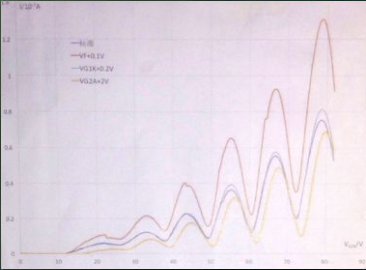
\includegraphics{lab2151_1.png}
    \caption{四条曲线对比图(仅供参考,实际图片请根据实验数据自行绘制)}
	\end{figure}

\subsection*{5.示波器自动测量}

\begin{figure}[H]
	\centering
		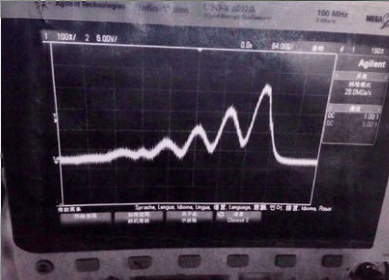
\includegraphics{lab2151_2.png}
	\end{figure}

\end{comment}
\fi
\end{document}